\chapter{Eksperyment na danych syntetycznych (MNIST)}

Do przetestowania pomysłu posłuży mi zbiór MNIST. Jest to zestaw odręcznie napisanych cyfr, które następnie zostały znormalizowane względem rozmiaru i wycentrowane. Każdy obrazek ma rozmiar 28x28 pikseli, mających wartości całkowite z przedziału [0, 255]. Na zbiór składa się 60 tys. danych treningowych i 10 tys. testowych. Przykładowe obrazki znajdują się na rysunku \ref{fig:mnist}.

\begin{figure}[h!]
    \centering
    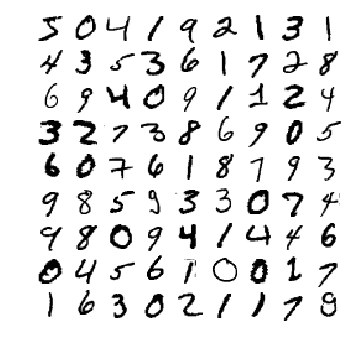
\includegraphics[width=0.5\textwidth]{images/mnist_v2}
    \caption{Przykładowe dane ze zbioru MNIST}
    \label{fig:mnist}
\end{figure}

\section{Mozliwości autoenkodera wariacyjnego} \label{sec:vae_oppo}

Chciałbym zacząć od sprawdzenia podstawowych własności autoenkodera wariacyjnego, przedstawionych w rozdziale \ref{sec:vae} W tym celu wytrenowałem modele o różnych rozmiarach reprezentacji ukrytej: 2, 5, 7, 20, 50. Następnie sprawdziłem jak radzą sobie z rekonstrukcją danych ze zbioru testowego oraz generowaniem nowych próbek. Wyniki prezentują się na rysunku \ref{fig:mnist_recon}. 

\begin{figure}[h!]
  \centering
  \begin{subfigure}[b]{0.7\linewidth}
    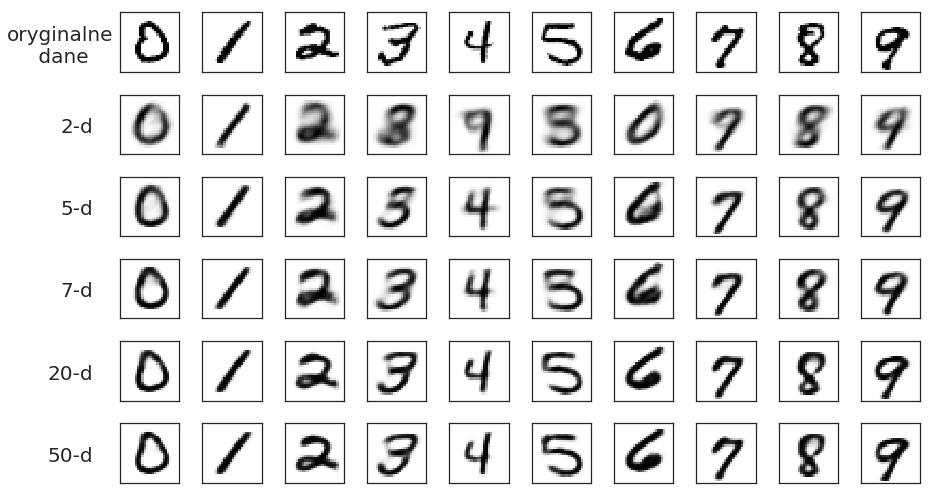
\includegraphics[width=1.0\textwidth]{images/mnist_recon_v3}
    \caption{}
  \end{subfigure}
  \begin{subfigure}[b]{0.7\linewidth}
    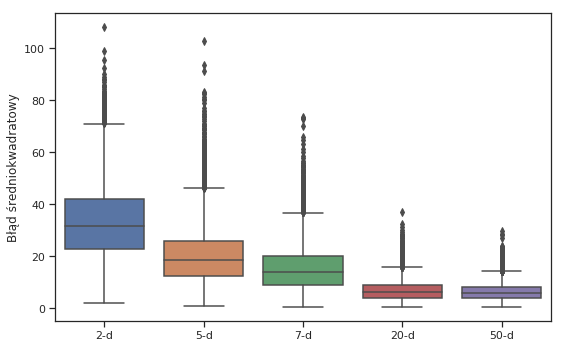
\includegraphics[width=1.0\textwidth]{images/vae_mse}
    \caption{}
  \end{subfigure}
  \begin{subfigure}[b]{0.7\linewidth}
    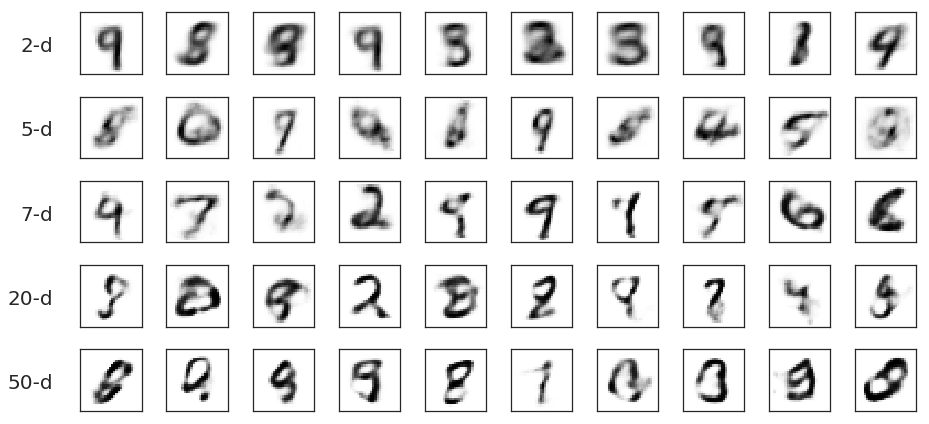
\includegraphics[width=1.0\textwidth]{images/mnist_gen_v2}
    \caption{}
  \end{subfigure}
  \caption{}
  \label{fig:mnist_recon}
\end{figure}

Ze względu na łatwość wizualizacji, do sprawdzenia jak dane reprezentowane są w przestrzeni ukrytej wybrałem model bazujący na wymiarze rozmiaru 2. Zdaję sobie sprawę, że rekonstrukcje w tym przypadku nie są najlepszej jakości, ze względu na zbyt ograniczoną ilość informacji możliwych do przekazania, ale zależy mi też na przedstawieniu podstawowych założeń. W tym celu na wykresie dla losowych próbek zaznaczyłem odpowiadające im średnie oraz odchylenia. Otrzymany rezultat widać na obrazku \ref{fig:mnist_2d}, gdzie można zauważyć opisane wcześniej własności wybranego modelu takie jak skoncentrowanie reprezentacji wokół $\vec{0}$ czy ciągłość przestrzeni.

\begin{figure}[h!]
    %\centering
    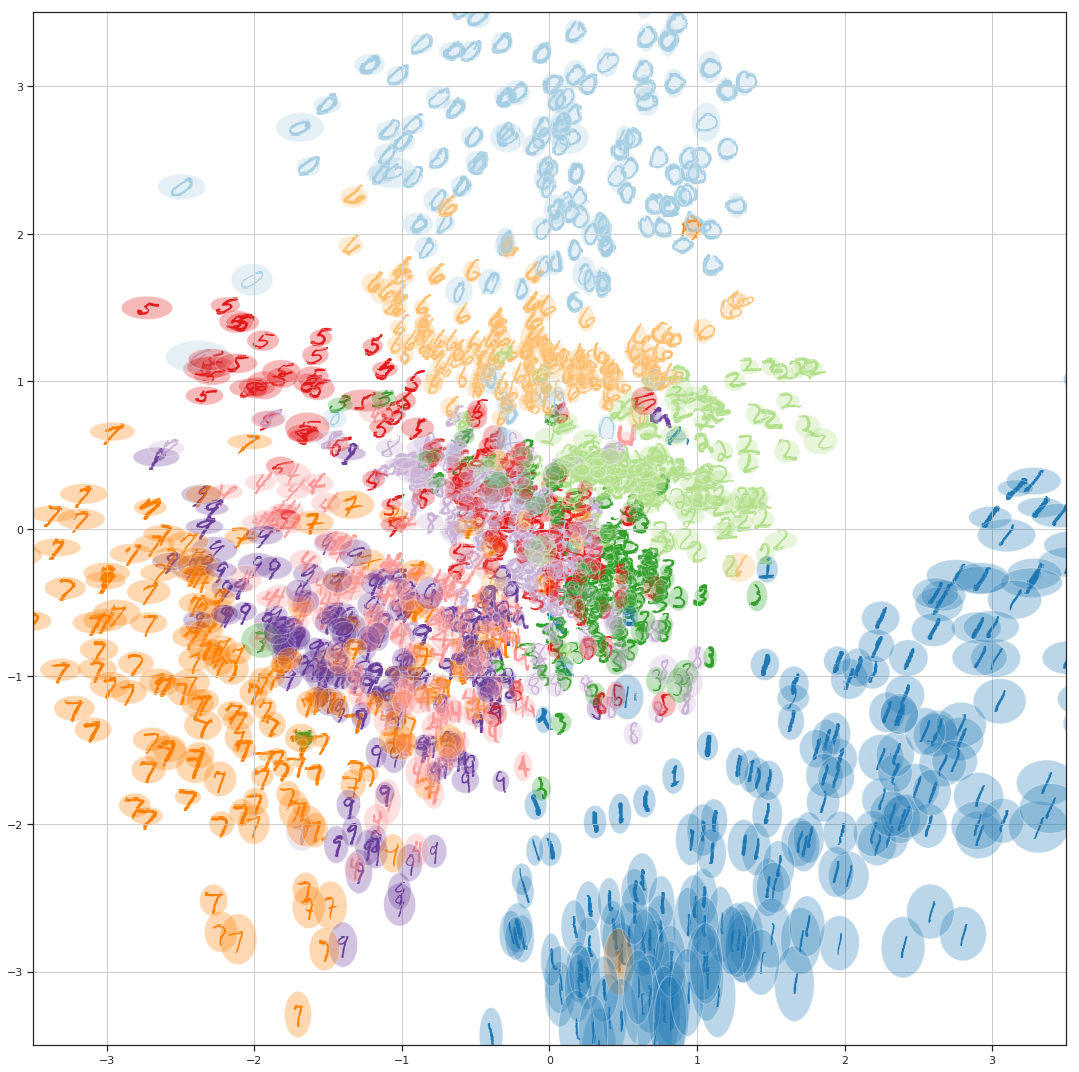
\includegraphics[width=1.2\textwidth,center]{images/mnist_2d}
    \caption{}
    \label{fig:mnist_2d}
\end{figure}

\section{Symulacja docelowego problemu}

W tym miejscu interesuje mnie odtworzenie oryginalnego problemu na prostszych danych, jakim jest właśnie zbiór MNIST. Pozwoli mi to stwierdzić sensowność skorzystania z wybranego modelu. Zakładam, że jeżeli eksperyment nie powiódłby się na łatwiejszych danych, to raczej nie powiedzie się również na tych skomplikowanych. Dodatkowo zyskam pewnego rodzaju doświadczenie z wybraną architekturą.

Przygotowana przeze mnie symulacja prezentuje się następująco. Zbiór danych składa się z trzech cyfr: 4, 5, 7, z czego 5 stanowi jedynie 1\% wszystkich próbek. Ma to odpowiadać rzadkości sytuacji patologicznych. Natomiast zadaniem jest stwierdzenie czy dana obserwacja jest cyfrą 5 czy nie.

Klasyfikacja odbywać się będzie na podstawie wartości funkcji straty dla autoenkodera wariacyjnego, którą można interpretować jako ograniczenie prawdopodobieństwa. Takie podejście wymaga ustalenia pewnego progu kategoryzacji, dlatego w tym miejscu będę prezentował krzywą ROC, która rozważa wszystkie sensowne wartości. Dodatkowo zaprezentuję dwa składniki błędu oddzielnie, przez co będzie można zaobserwować, który z nich ma największy wpływ.

Na podstawie wniosków z rozdziału \ref{sec:vae_oppo} wybrałem rozmiar warstwy ukrytej równy 10. Wyniki zaprezentowane są na rysunku \ref{fig:mnist_compare} oraz \ref{fig:mnist_roc}.

\begin{figure}[h!]
    \centering
    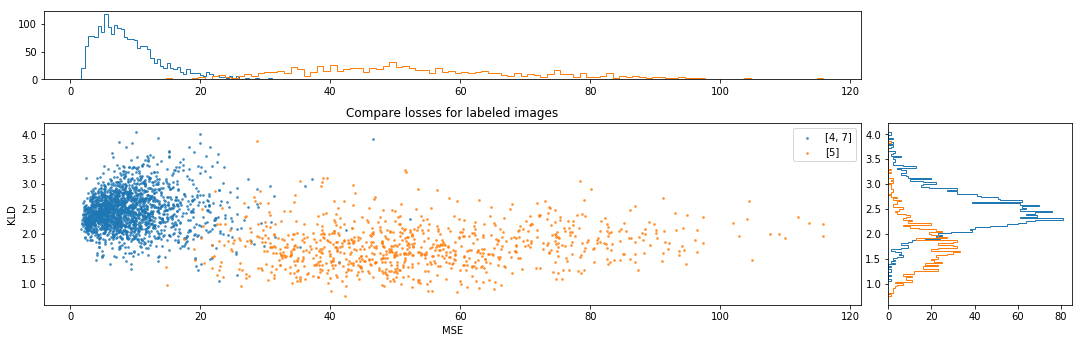
\includegraphics[width=1.0\textwidth]{images/mnist_compare}
    \caption{}
    \label{fig:mnist_compare}
\end{figure}

\begin{figure}[h!]
    \centering
    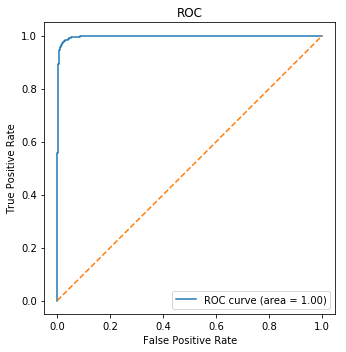
\includegraphics[width=0.5\textwidth]{images/mnist_roc}
    \caption{}
    \label{fig:mnist_roc}
\end{figure}

\section{Wnioski}

Na podstawie otrzymanych wyników mogę stwierdzić, że eksperyment się powiódł. W przypadku danych MNIST udało się sklasyfikować dane, które są rzadkie i stanowią jedynie odsetek wszystkich. Jest sens w takim razie w użyciu tego modelu dla już prawdziwych danych.
